\section{Introducción}

\begin{frame}{Motivación y audiencia}
  \begin{itemize}
    \item Fin del escalado de Dennard: más núcleos en lugar de frecuencias crecientes.
    \item Curso de Redes, Arquitectura y Comunicaciones dirigido a estudiantes de la Facultad de Ciencias Matemáticas.
    \item Objetivo: mostrar patrones prácticos de paralelismo con énfasis en código real y decisiones de diseño.
  \end{itemize}
\end{frame}

\begin{frame}{Imperativo del paralelismo}
  \begin{itemize}
    \item Multinúcleo obliga a dividir trabajo en flujos simultáneos para servidores, procesamiento de paquetes y cómputo intensivo.
    \item Lenguajes presentan filosofías distintas: C ofrece control de bajo nivel; Python prioriza productividad y simplicidad.
    \item El diseño debe balancear latencia, throughput y complejidad de implementación.
  \end{itemize}
\end{frame}

\begin{frame}{Contexto visual}
  \begin{figure}
    \centering
    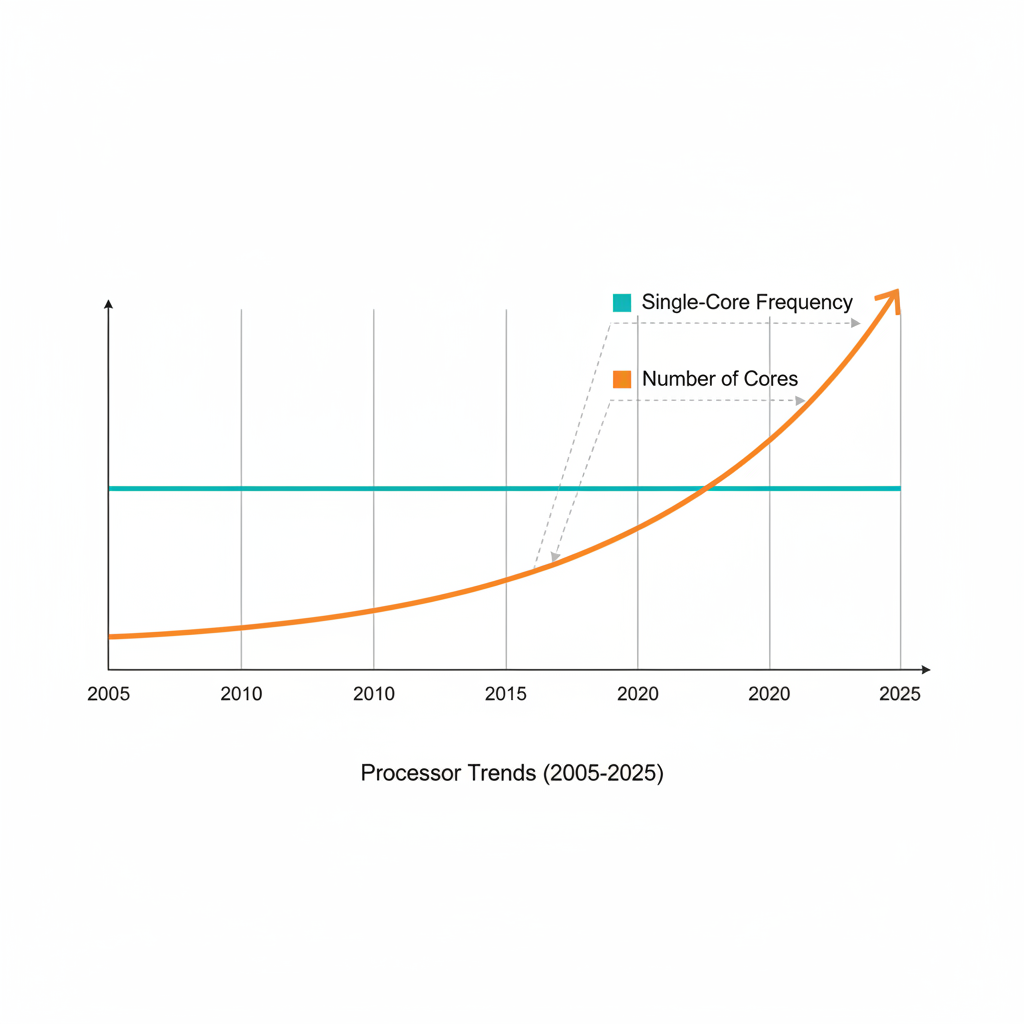
\includegraphics[height=0.6\textheight]{img/01-frecuencia-vs-nucleos.png}
    \caption{Crecimiento de la frecuencia de un solo núcleo frente al número de núcleos.}
  \end{figure}
\end{frame}
